\documentclass{beamer}
\usetheme{Warsaw}
\usepackage[utf8]{inputenc}
\usepackage[T1]{fontenc}
\usepackage{mathtools}


\title[DNNLM]{Deep Neural Network Language Models}
\author[A. Peyrard, T. Cantenot]{Alex Peyrard, Thierry Cantenot}
\institute{Shanghai JiaoTong University}
\date{\today}

\setbeamertemplate{blocks}[rounded][shadow=false]
\addtobeamertemplate{block begin}{\pgfsetfillopacity{0.8}}{\pgfsetfillopacity{1}}
\setbeamercolor*{block title example}{fg=blue!150, bg= blue!10}
\setbeamercolor*{block body example}{fg= black, bg= blue!5}

\addtobeamertemplate{footline}{\insertframenumber/\inserttotalframenumber}


\begin{document}
\begin{frame}[plain]
	  \titlepage
\end{frame}

\begin{frame}{Introduction}
	\begin{center}
		Deep Neural Networks Language Models\\
		Ebru Arısoy, Tara N. Sainath, Brian Kingsbury, Bhuvana Ramabhadran\\
		IBM T.J. Watson Research Center\\
		Yorktown Heights, NY, 10598, USA\\
		\{earisoy, tsainath, bedk, bhuvana\}@us.ibm.com
	\end{center}
\end{frame}

\begin{frame}{What is a Language Model?}
	\begin{quote}
		A statistical language model assigns a probability to a sequence of m words $P(w_1,\ldots,w_m)$ by means of a probability distribution. \\ \flushright\emph{Wikipedia -- Language Models}
	\end{quote}
\end{frame}

\begin{frame}{What is a Neural Network ?}
\begin{figure}[!ht]
	\centering
	\rule{0cm}{0cm}
    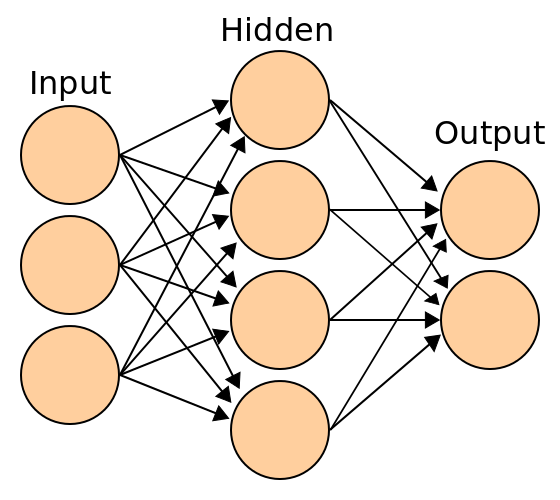
\includegraphics[width=0.5\linewidth]{./images/ANN.png}
	\caption{A neural network}
\end{figure}
\end{frame}

\begin{frame}{What is a Neural Network?}
	A neuron is defined by :
	\begin{itemize}
		\item Bias
		\item Weight
		\item Activation function
	\end{itemize}
	\vspace{5mm}
	The bias and weight are updated during training. The activation function is chosen when the network is first designed.
	\begin{exampleblock}{Node output}
	\[f(\sum\limits_{i}W_{i}x_{i} + b)\]
	\end{exampleblock}
\end{frame}

\begin{frame}{Activation function}
	The activation function often if the sigmoid or hyperbolic tangent function.
	\begin{center}
		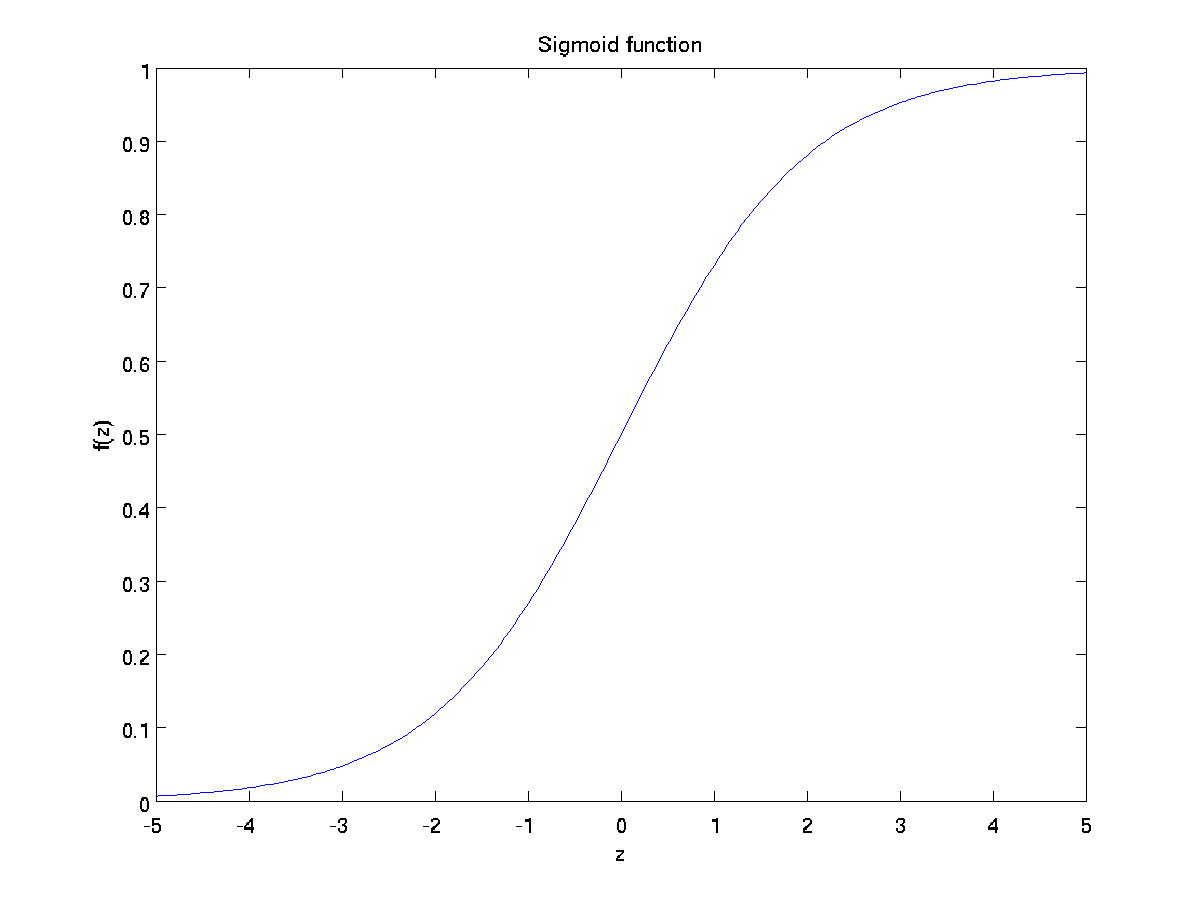
\includegraphics[scale=0.28]{images/sigmoid.png}
		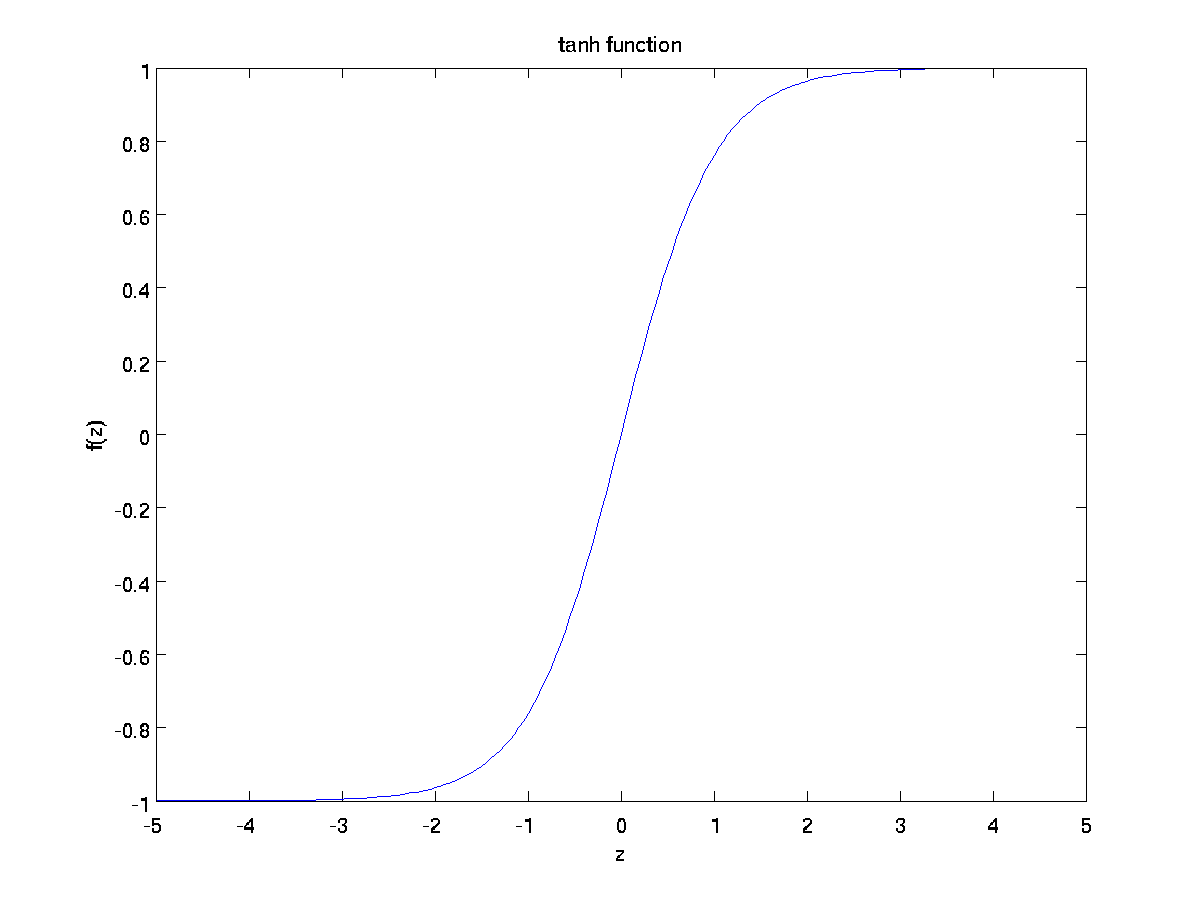
\includegraphics[scale=0.28]{images/tanh.png}
	\end{center}
\end{frame}

\begin{frame}{Why Neural Network Language Modeling?}
	The state of the art uses n-grams
	\begin{itemize}
		\item Data spareness requires smoothing to avoid small or zero probabilities for some valid word sequences
		\item Discrete nature $\rightarrow$ generalization is hard. No notion of word similarity
	\end{itemize}
	\vspace{5mm}
	The neural network language model embeds words in a continuous space. The aim is to use appropriate data for training so that similar words are close in the continuous space, thus obtaining better results for unseen n-grams.
\end{frame}

\begin{frame}{Feed-forward NNLM architecture}

\begin{figure}[!htb]\centering
    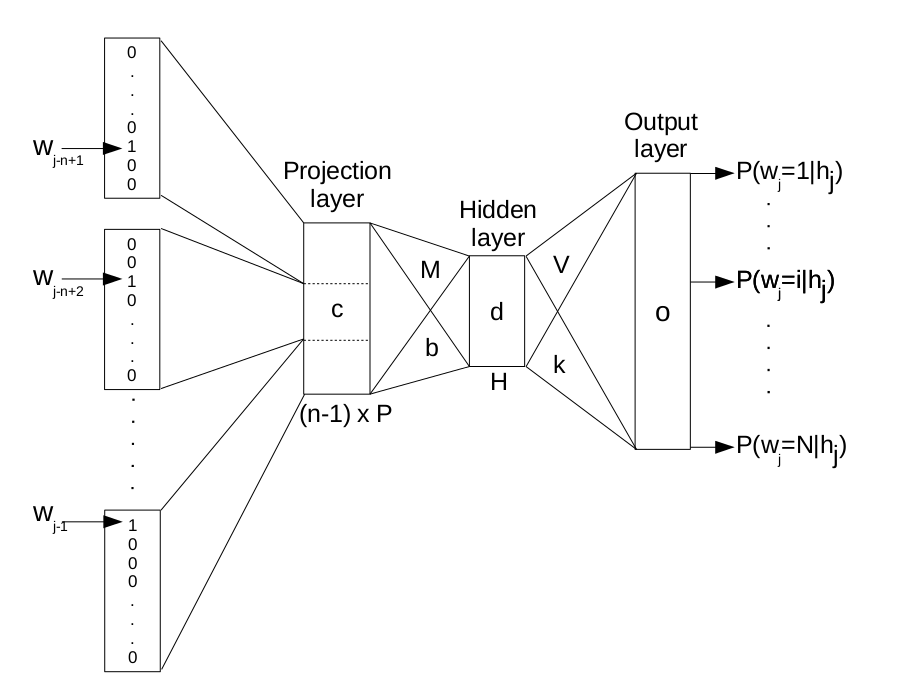
\includegraphics[width=0.8\linewidth]{./images/architecture.png}
    \caption{Feed-forward neural network language model architecture}\label{diagram:architecture}
\end{figure}

\end{frame}


\begin{frame}{Feed-forward NNLM architecture}

\begin{exampleblock}{Neural network's operations}
\begin{equation}
\left.\begin{aligned}
    &d_j = tanh(\sum\limits_{l=1}^{\text{\tiny{$(n-1) \times P$}}}{M_{jl} \times c_l + b_j}) \qquad \text{\small{$\forall j = 1, \ldots, H$}}&\\
    &o_i = \sum\limits_{j=1}^{H}{V_{ij} \times d_j + k_i} \qquad \text{\small{$\forall i = 1, \ldots, N$}}&\\
    &p_i = \frac{exp(o_i)}{\sum\limits_{r=1}^{N}{exp(o_r)}} = P(w_j = i | h_j)&\\
\end{aligned}\right.
\end{equation}
\end{exampleblock}

where $M$ and $V$ are the \textbf{weight matrices} between the projection and hidden layers and between the hidden and output layers \\and $b_j$ and $k_i$ are the hidden and output layer \textbf{biases} respectively.

\end{frame}


\begin{frame}{Feed-forward Deep NNLM architecture}

The DNNLM has the same architecture as a NNLM but with \textbf{several hidden layers of nonlinearities}.
\newline
\newline
In the acoustic modeling community, DNNs have proven to be competitive with the well-established Gaussian mixture model:
\newline
\begin{center}
\textbf{How well DNNs can perform in language modeling?}
\end{center}

\end{frame}


\begin{frame}{Experimental setup}

\textbf{Baseline ASR system}
\newline
\newline
900K sentences (23.5M words) from 1993 WSJ text with verbalized punctuation from the CSR-III: \\
\begin{itemize}
    \item 2,439 unique utterances (46,888 words) as \textit{evaluation set}.
    \item 977 utterances (18,279 words) as \textit{development set}.
    \item The rest as \textit{training set}.\\
\end{itemize}

Comparison with the state-of-the-art \textbf{model M language model}.
\newline
\newline
After rescoring, the \textbf{baseline WER} is $20.7\%$ on the held-out set and $22.3\%$ on the test set.

\end{frame}

\begin{frame}{Experimental setup}

\textbf{DNN language model set-up}
\newline
\newline

\end{frame}

\begin{frame}{Results}
	\begin{figure}[!htb]
		\centering
	    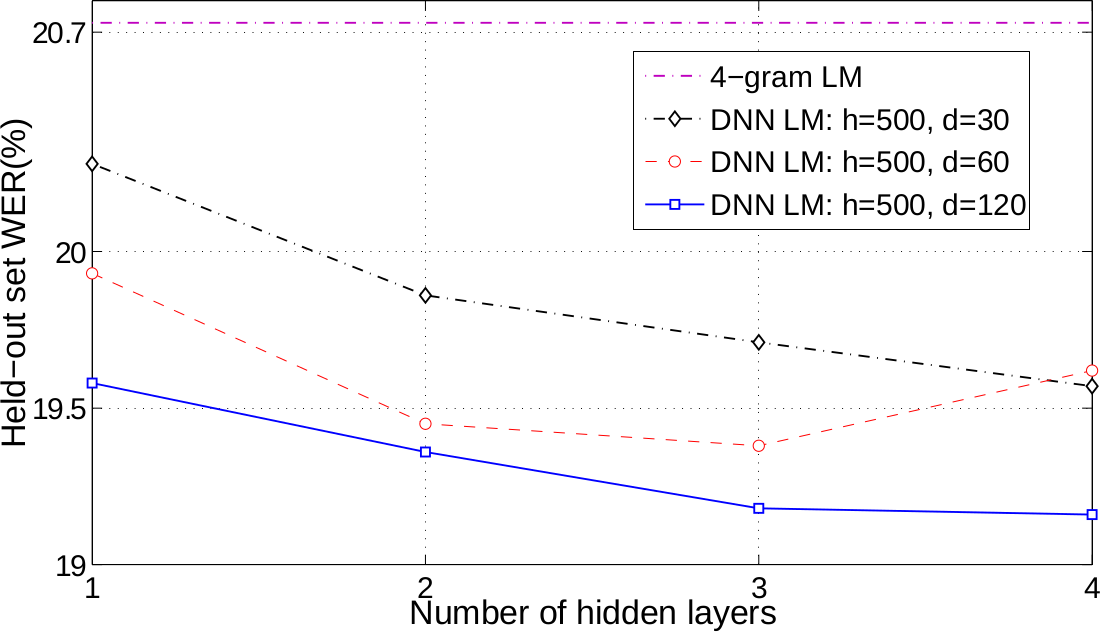
\includegraphics[width=0.8\linewidth]{./images/results1.png}
	    \caption{WER function of number of hidden layers}
	\end{figure}
\end{frame}

\begin{frame}{Results}
	\begin{figure}[!htb]
		\centering
			\begin{minipage}{0.45\textwidth}
				    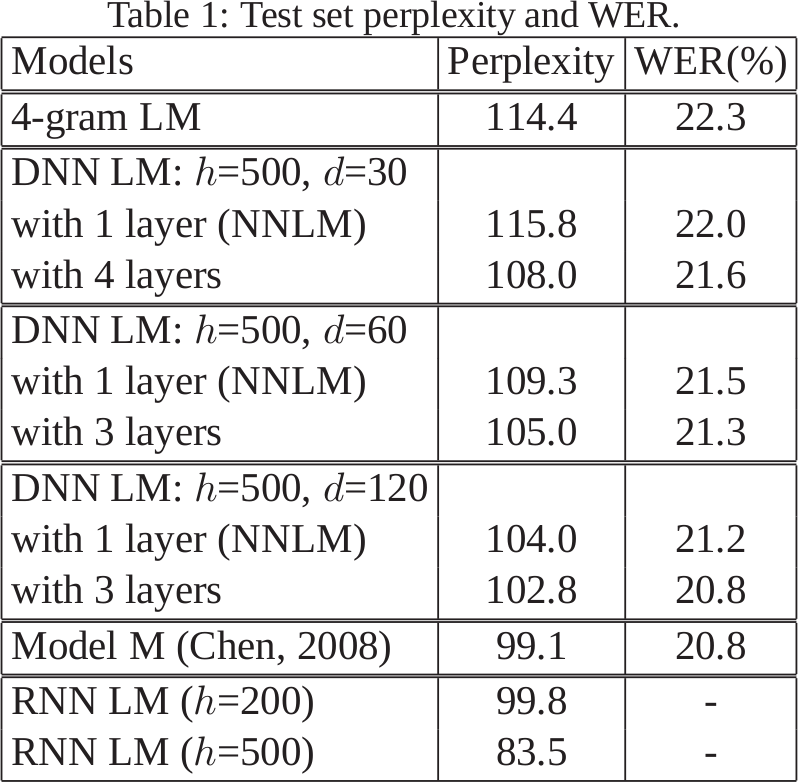
\includegraphics[width=\linewidth]{./images/results2.png}
			\end{minipage}
			\hspace{5mm}
			\begin{minipage}{0.45\textwidth}
				    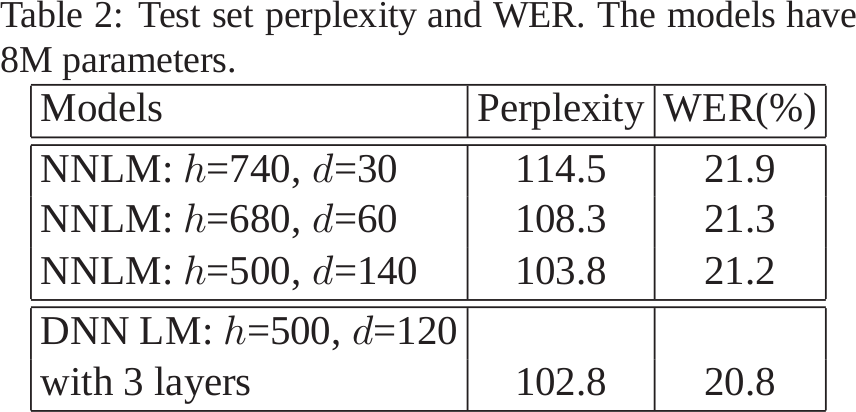
\includegraphics[width=\linewidth]{./images/results3.png}
			\end{minipage}
	\end{figure}
\end{frame}

\begin{frame}{Results}
	\begin{figure}[!htb]
		\centering
			\begin{minipage}{0.45\textwidth}
				    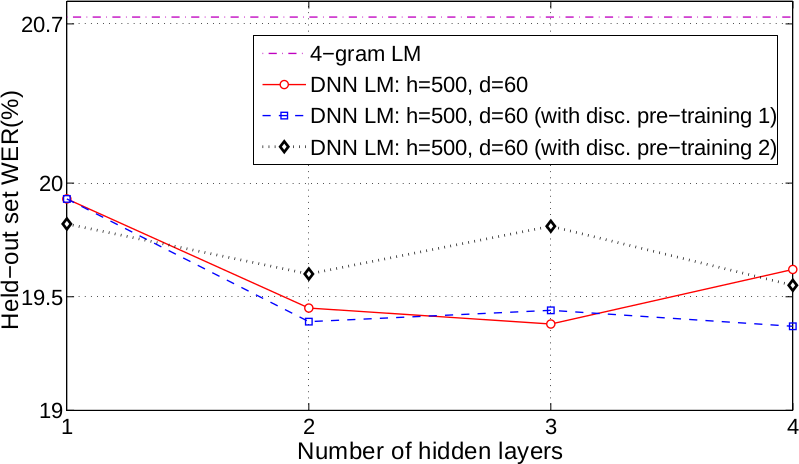
\includegraphics[width=\linewidth]{./images/results4.png}
			\end{minipage}
			\hspace{5mm}
			\begin{minipage}{0.45\textwidth}
				    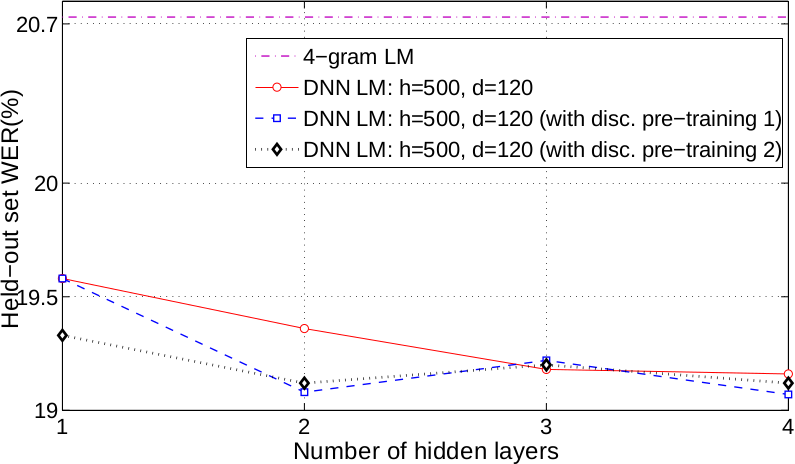
\includegraphics[width=\linewidth]{./images/results5.png}
			\end{minipage}
		\caption{WER function of number of hidden layers}
	\end{figure}
\end{frame}

\end{document}
